\title{LEZIONE 1 9/03/2020}\newline
\textbf{link} \href{https://web.microsoftstream.com/video/6164a9b1-4d0a-4f37-a279-2e0ec1e8ca25?list=user&userId=faa91214-a6f5-40d7-8875-253fd49b8ce1}{clicca qui}
\section{SLIDE: Introduzione al corso}
Slide: \url{../pdf/IntroduzioneCorsoFdA-2019.2020.pdf}.
\subsection{Informazioni generale}
\textbf{[0-10]}\;\newline
Prof. Alberto Leva \newline
Il materiale didattico è distribuito su Beep e sulla \href{http://home.deib.polimi.it/leva/}{pagina del corso}.\newline
Le slide e il materiale del corso non è sufficiente, bisogna prendere appunti e studiare dai testi.\newline
Non ci sono prove in itinere.
\subsection{Concetti preliminari}
\textbf{[11]}\;
\newline\textbf{[12]}\;
\newline\textbf{[13]}\;
\newline\textbf{[14]}\;
\newline\textbf{[15]}\;
\newline\textbf{[16]}\;
\newline\textbf{[17]}\;
\newline\textbf{[18]}\; Laboratorio: due transistor (marroni) non in contatto diretto, ma legati da una barretta di rame (azzurra), ci sono tre sensori di temperatura (blu), due sui transistor e uno sulla barretta (non si vede), c'è anche una ventola che può essere azionata o meno. Lo scopo è controllare la temperatura della barretta agendo su uno dei due transistor, mentre l'altro ha lo scopo di rappresentare un disturbo.
\newline\textbf{[19]}\;
\newline\textbf{[20]}\;
\newline\textbf{[21]}\;
\newline\textbf{[22]}\;
\subsection{Prerequisiti, motivazione e collocamento del corso}
\textbf{[23]}\;
\newline\textbf{[24]}\;
\newline\textbf{[25]}\;
\newline\textbf{[26]}\;
\newline\textbf{[27]}\; Struttura del corso. Nozioni base da sapere: derivate, integrali, invertire un matrice, autovalori e autovettori. 
\subsection{Relazione fra automatica e informatica}
\textbf{[28]}\;
\newline\textbf{[29]}\;
\newline\textbf{[30]}\;
\newline\textbf{[31]}\;
\newline\textbf{[32]}\;
\newline\textbf{[33]}\;
\newline\textbf{[34]}\;
\newline\textbf{[35]}
\newpage
\section{Il problema del controllo}
\subsection{Concetti fondamentali}
[immagine dagli appunti del prof]
\begin{center}
    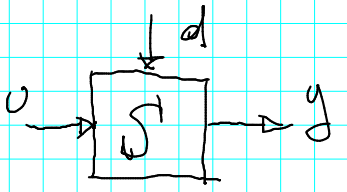
\includegraphics[height=3cm]{../lezione1/img1.PNG}
\end{center}
$S$: sistema da controllare. \newline
$U$: variabili di controllo o in generale variabili di ingresso. Da notare è che per esempio anche una pompa che possiamo comandare e che tira fuori acqua dal nostro sistema è una variabile di ingresso perchè la controlliamo, nonostante la massa fisica dell'acqua esca.\newline
$y$: variabili d'uscita.\newline
$w$: andamento desiderato di $y$ o segnale di riferimento o set point.\newline
$d$: disturbi.\newline
L'obbiettivo è che $y$ sia il più possibile uguale a $w$ nonostante $d$ e nonostante una conoscenza potenzialmente imperfetta di $S$.
\subsection{Strategie di controllo}
\subsubsection{Controllo in anello aperto (AA)}
[immagine dagli appunti del prof]
\begin{center}
    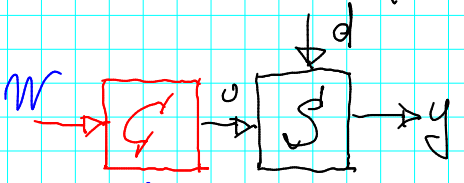
\includegraphics[height=3cm]{../lezione1/img2.PNG}
\end{center}
$C$: controllore.\newline
Il controllore decide l'andamento di $U$ sulla base di $w$. Il controllore non sa cosa succede in $y$ e non conosce $d$.\newline
Questo approccio funziona se il legame $U \rightarrow y$ è esattamente noto e non ci sono disturbi $d$.\newline
\subsubsection{Controllo in anello aperto (AA) con compensazione del disturbo misurabile}
[immagine dagli appunti del prof]
\begin{center}
    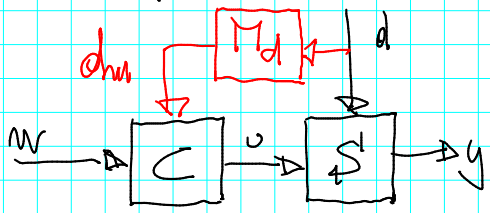
\includegraphics[height=3cm]{../lezione1/img3.PNG}
\end{center}
$M_d$: misuratore del disturbo.\newline
$d_m$: misura del disturbo $d$.\newline
Il controllore in questo caso non vede $y$, ma vede $d$ (o meglio $d_m$).\newline
Questo approccio funziona se il legame $(U,d) \rightarrow y$ è esattamente noto e se $d_m = d$, cioè se la misura del disturbo è corretta.
\subsubsection{Controllo in anello chiuso (AC) o in retroazione o Feedback}
[immagine dagli appunti del prof]
\begin{center}
    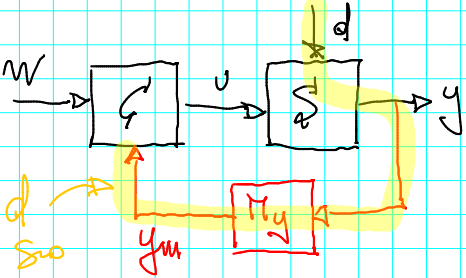
\includegraphics[height=3cm]{../lezione1/img4.PNG}
\end{center}
$M_y$: misuratore dell'uscita.\newline
$y_m$: misura dell'uscita $y$.\newline
Questo sistema può contrastare i disturbi ed errori di modello anche senza conoscerli, infatti il controllore ne vede gli effetti tramite $y_m$.\newline
Naturalmente occorre sempre che $y_m = y$, se la misurazione è sbagliata non si può fare nulla. Facciamo notare che le misurazioni sono particolarmente importanti, non lavoriamo con le grandezze vere e proprie, ma con le loro misurazioni.
\subsubsection{Controllo in anello chiuso (AC) con compensazione del disturbo}
[immagine dagli appunti del prof]
\begin{center}
    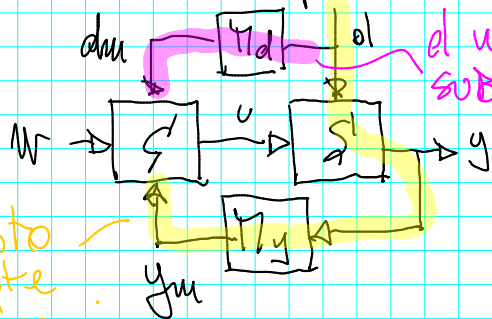
\includegraphics[height=3cm]{../lezione1/img5.PNG}
\end{center}
Questo approccio è come il caso precedente ma più pronto nel reagire ai disturbi $d$. Nel caso precedente potevamo correggere gli effetti di un disturbo osservando i suoi effetti sull'uscita, in questo caso, invece, si reagisce in maniera preventiva ai disturbi, cioè non appena viene rilevato un disturbo il controllore può già andare a contrastarlo senza dover aspettare che questo influenzi l'uscita.\newline
\textbf{oss.} La precisione di $M_d$ conta meno di quella di $M_y$.
\subsubsection{Esempio}
[immagine dagli appunti del prof]
\begin{center}
    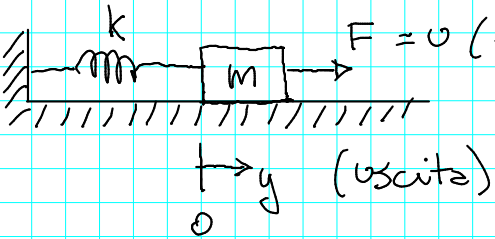
\includegraphics[height=3cm]{../lezione1/img6.PNG}
\end{center}
Abbiamo una guida su cui scorre una massa $M$ attaccata con una molla di costante elastica $k$. La massa viene spinta da una forza $F = U$ (che è l'ingresso con cui possiamo interagire col sistema). La $y$ (uscita) del sistema è la posizione della massa sulla guida, che vale $0$ quando il sistema è a riposo.
\[
    F_{molla} = -ky \;\;\;\;\;\;\;\;\;\;\;\;\;\;\;\;\;\;\;\;F_{attrito} = - h \frac{d}{dt}y = -h \dot{y}
\]
Analiziamo ora questo sistema nel caso in cui sia in equilibrio (cioè fermo) e nel caso in cui sia in movimento.
\subsubsection*{Modello statico}
Per prima cosa vediamo un \textbf{modello statico (all'equilibrio)} di questo sistema:\newline
In un modello statico la velocità è nulla, e quindi la $F_{attrito} = 0$ e $F + F_{molla} = 0$, che diventa $F-k \bar{y} = 0$, dove per $\bar{y}$ si intende il valore di $y$ in stato di equilibrio, e dunque $\bar{y} = \frac{F}{k}$.\newline
Quindi se voglio $y = y^o$, dove per $y^o$ si intende un $y$ desiderato, dovrò applicare una forza $F = k y^o$.\newline
\newline
Analiziamo ora il sistema con un controllo in \textbf{AA}, supponendo che la costante elastica della molla sia $k = k_n + \Delta k$, dove $k_n$ è detto $k$ nominale e $\Delta k$ rappresenta un possibile errore di modello a noi sconosciuto.\newline
Applicando quindi $F = k_n y^o$, otterrò $y = \frac{F}{k_n + \Delta k} = \frac{k_n}{kn + \Delta k} y^o$. Quindi si può avere un errore di modello dovuto a quel $\Delta k$, che provoca un errore di controllo, cioè un errore in cui l'uscita effettiva non è esattamente l'uscita che volevamo: $y \neq y^o$.\newline
\[
    \text{Errore nel modello ($\Delta k$) $\Longrightarrow$ errore nel controllo ($y \neq y^o$)}\;
\]
\newline
Analiziamo ora il sistema con un controllo in \textbf{AC}.\newline
Posso decidere di applicare una forza $F = \alpha (y^o -y)$, con $\alpha>0$. Il termine $(y^o - y)$ rappresenta l'errore, (quello che voglio - quello che ho). $F$ è la variabile di controllo ed è proporzionale ($\alpha$) all'errore.\newline
Questo è un esempio di applicazione di controllo ad anello chiuso.\newline
Con questo approccio ottengo $y = \frac{F}{k_n + \Delta k} = \frac{\alpha (y^o - y)}{k_n + \Delta k}$ e continuando i conti si arriva a $\frac{y - y^o}{y^o} = \frac{k}{k+\alpha}$, dove il termine $\frac{y-y^o}{y^o}$ prende il nome di errore normalizzato. Se $k = k_n$ non ho errore, però con $\alpha$ abbastanza grande posso rendere l'errore piccolo a piacere (con possibili problemi di stabilità di cui parleremo più avanti).\newline
\newline
Quindi:
\begin{itemize}
    \item  il controllo in AA è basato sul modello (usa $k_n$); l'errore è nullo se il modello è esatto, se no non si può contrastare l'incertezza.
    \item il controllo in AC è basato su misure (usa $y^o-y$); l'errore può essere reso piccolo a piacere.
\end{itemize}
\subsubsection*{Modello dinamico}
Vediamo ora il \textbf{modello dinamico}:
Partiamo dalla famosa formula "$\text{massa} \cdot \text{accellerazione}\; = \sum \text{forze}$".\newline
Quindi $m \cdot \ddot{y} = F - ky - h \dot{y}$, cioè $m \ddot{y}(t) + h \dot{y}(t) + k y(t) = F(t)$.\newline
\newline
Nel caso di un sistema con controllo in \textbf{AA}, $F(t)$ non dipende da $y(t)$ e quindi l'integrale generale non cambia qualunque sia $F(t)$.\newline
\newline
Nel caso di un sistema con controllo in \textbf{AC}, se, per esempio, $F(t) = \alpha(y^o(t) -y(t)) + \beta \dot{y}(t)$, ovvero se faccio dipendere la forza istante per istante, devo scrivere che $m \ddot{y}(t) + h \dot{y}(t) + k y(t) = \alpha(y^o(t) - y(t) ) + \beta \dot{y}(t)$, cioè $m \ddot{y}(t) + (h - \beta) \dot{y}(t) + (k + \alpha)y(t) = \alpha y^o(t)$. Agendo su $\alpha$ e $\beta$ sto cambiando il polinomio caratteristico dell'equazione differenziale e quindi sto cambiando l'integrale generale. L'integrale generale dipende dai parametri di controllo $\alpha$ e $\beta$.\newline
\newline
[immagine dagli appunti del prof]: schema a blocchi (verrà spiegato meglio più avanti) dell'esempio appena fatto.
\begin{center}
    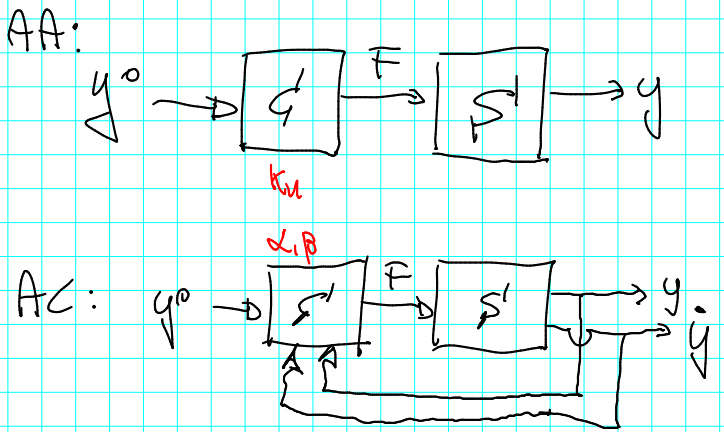
\includegraphics[height=3cm]{../lezione1/img7.PNG}
\end{center}